
\chapter{Introduction}


\section{Background}
% One of the challenges in the transition from traditional energy to sustainable energy like solar and wind is the fluctuation of these energy sources. An electric grid could become destabilized if non-dispatchable renewable energy exceeds 20\% of the energy-generation capacity without energy storage \cite{Weber2011}. The solution for such problems involves the large scale application of energy storage system as a buffer. 

Buoyancy driven bubbly flow widely exists in the chemical industry. In this study, we focus on its application in electrochemical cells.

% An ideal equipment for large-scale grid storage requires
% durability for large numbers of charge and discharge cycles as
% well as calendar life, high round-trip efficiency, and ability
% to respond rapidly to changes in load or input, and reasonable
% capital costs \cite{Weber2011}.

Electrochemical cells are more and more used in the chemical industry as a means for efficient energy storage as well as the production of gases valuable in the various chemical engineering process, such as hydrogen, chlorine \cite{Sokolichin2004}, etc. Compared with supercapacitors and solid-state batteries,
electrochemical cells store more energy and deliver more power. Compared with compressed air and pumped hydro energy storage, electrochemical cells have less environmental impacts and are less demanding in terms of geography \cite{Ke2018}.

\section{Buoyancy-driven bubbly flow in electrochemical cells}

% Normal setups of electrochemical cells include hydrogen-bromine, vanadium, water electrolysis, etc. A sketch of typical electrochemical cells are shown in figure \ref{flow_cell}:

\begin{figure}[H]
\centering
\begin{subfigure}{.4\textwidth}
  \centering
  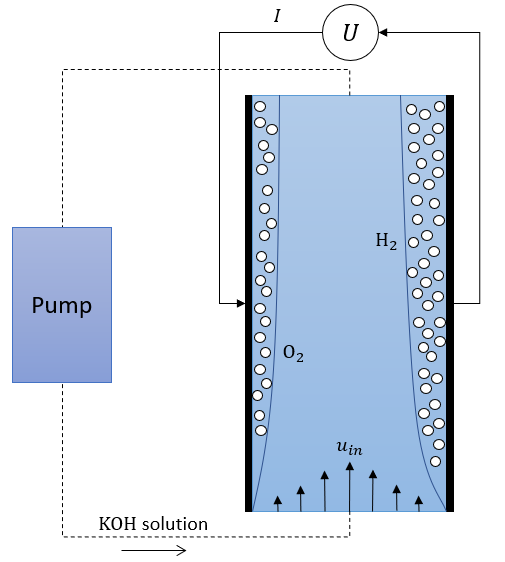
\includegraphics[width=1\linewidth]{forcedflowsketch.png}
  \caption{The forced flow setup, an inlet velocity is given by the pump at the bottom of the channel}
  \label{forcedsetup}
\end{subfigure}%
\begin{subfigure}{.4\textwidth}
  \centering
  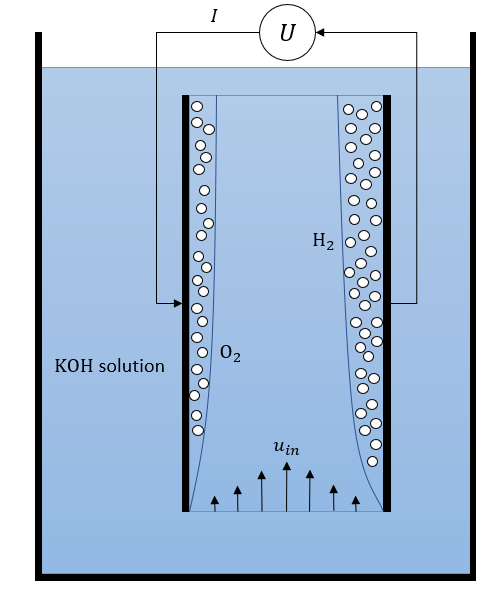
\includegraphics[width=1\linewidth]{buoyancydrivenflowsketch.png}
  \caption{The natural flow setup, the flow is purely driven bu the rising bubbles}
  \label{naturalsetup}
\end{subfigure}
\caption{Sketches for two different setups of buoyancy driven bubbly flow}
\label{sketchcell}
\end{figure}

Buoyancy-driven bubbly flows exist in various kinds of electrochemical cells. One typical application is water electrolyzer. Figure \label{sketchcell} gives two different kinds of commonly seen setup. \ref{forcedsetup} is a forced flow setup, where the flow is partly driven by the bubbles and partly by the fed flow at the bottom. \ref{naturalsetup} is a natural flow setup, since the flow is purely driven by the bubbles.



Besides the setup in figure \ref{sketchcell}, there are also setups with membranes for applications like water electrolysis and chlorate \cite{Alexiadis2012b}. 

\begin{figure}[H]
    \centering
    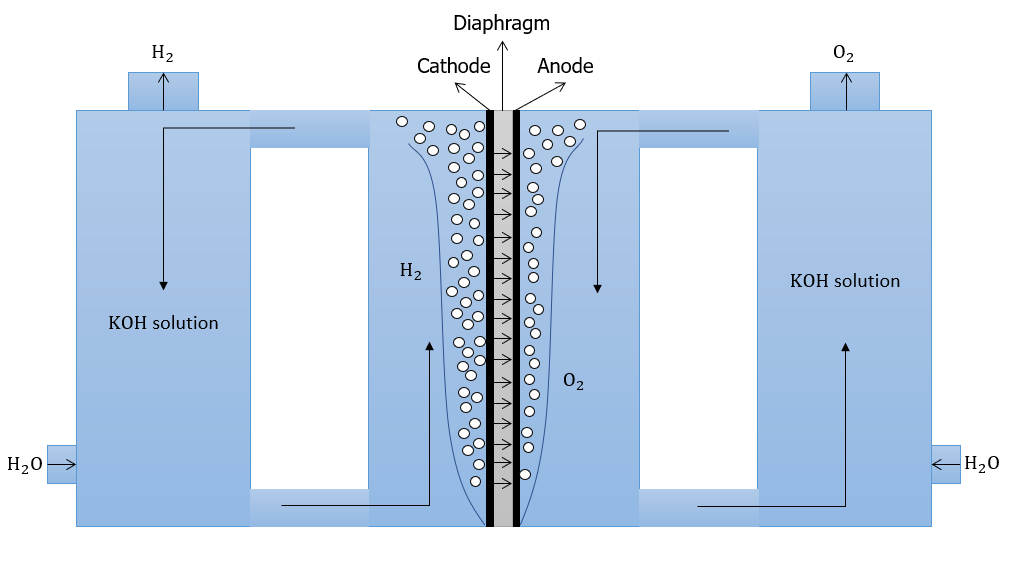
\includegraphics[scale=0.6]{Circulatingsketch.png}
    \caption{A sketch for buoyancy driven circulating bubbly flows}
    \label{vertical}
\end{figure}


In this circulating flow setup, the bubbles are generated from the electrode surface placed between two vertical channels, and the electrons are transferred through the diaphragm in the middle. While the bubbles are free to leave the channel when reaching the top, the liquid dragged by the rising bubbles is trapped inside the channel, thus forming a circulating flow. The area where liquid flows downward is called downcomer.

\section{Problem Statement}

While the efficiency of an electrochemical cell can be crucial for its success in commercial applications, the involvement of various types of gases significantly complicates the design and optimization process, since the evolution of gas exhibits some characteristics which are not typical of electrode processes in general \cite{Energy}. Therefore, studying the complex phenomena in the electrochemical cell could provide guidance for future design.

In this work, the focus is put on the numerical modelling of a buoyancy-driven circulating bubbly flow. CFD is used for the study of this research question. A numerical multiphase flow model is used to simulate the buoyancy-driven bubbly flow respectively in a vertical channel and a circulating channel in COMSOL. The results from the vertical channel simulation can be used for validation by comparing with results from other literature. Also we need the simulation results in the circulating channel to shed light on the impact of channel width and current density.


\section{Document Structure}
In Chapter 2, the basic theory for the modelling of bubbly flow in electrochemical cells is discussed, including all the simplifications made in the model, and the several types of numerical models that are frequently used today for the simulation of multiphase flow. Additionally, a literature review covering a series of works involving both simulation and modelling is given.

In Chapter 3, a numerical model done in a vertical channel (forced convection without recirculation flow) previously proposed by Wedin et al. \cite{Wedin2001} is presented, then also tested by \cite{Schillings2015a}. It is tested again in this work and compared with the experimental data from \cite{Boissonneau2000} to make sure that we can reproduce the results in those previous work. 

Chapter 4 presents the model of circulating flow and analysis, including the parametric study and the comparison with analytical solutions.

Finally, chapter 5 discusses the conclusions, the limitations of the current model, as well as the recommendation for future works.